\section{Simulations Experiments}
\label{sec:simulationexperiments}

This section presents the experimental results of the simulations of our proposed \ac{REACT} method. The entire framework is implemented in C++ to ensure computational efficiency and is integrated with ROS to facilitate modularity and deployment on real-world robots. Furthermore, the \ac{OMPL} library \cite{ompl} is utilized to compute the shortest paths using the RRT* algorithm.  

\subsection{Simulation experimental setup}
The path planner is implemented for a BlueROV2. A \ac{MPC} approach accounts for model constraints and provides the optimal control input $\mathbf{u}^{ref} \in \mathbb{R}^4$, where $\mathbf{u}^{ref} = [F_x, F_y, F_z, M_z]^T$ represents the forces in the $X$, $Y$, and $Z$ directions, and the moment about the $Z$-axis. The goal is to follow the desired reference trajectory $\mathbf{x}^{ref} \in \mathbb{R}^6$, where $\mathbf{x}^{ref} = [x_{ref}, y_{ref}, z_{ref}, \psi_{ref}]^T$ contains the reference position ($x_{ref}$, $y_{ref}$, $z_{ref}$) and the reference yaw angle $\psi_{ref}$. For further details about the controller and model, the reader is referred to \cite{amergp}. The entanglement-aware path planner provides $\mathbf{x}^{ref}$ in real time, ensuring the BlueROV2 avoids obstacles while following the desired trajectory. 

We perform a comparative analysis of the proposed \ac{REACT} method and a baseline conventional \ac{CPP} (FC-Planner \cite{feng2024fc}), which does not explicitly handle entanglement. 

The simulation setup uses a 1/10-scale pipe structure based on the model described in \cite{feng2024fc}. The simulated onboard camera has a field of view of 70 degrees. The tether constraint is implemented by specifying a maximum allowable tether length of \(L_{\text{max}} = 10\) meters. Note that the resulting planned trajectories are geometrically identical to those in the full-scale environment, simply scaled down proportionally. The primary motivation for using the scaled model is to accelerate simulation runs while preserving the validity of the results.

Coverage is computed in a manner similar to \cite{amer2023visual}. At each time step, the position and orientation of the camera are used to determine which triangles in the environment mesh are visible. A triangle is marked as visible if its centroid is within the inspection range, its surface normal faces the camera, and its projection lies within the camera's field of view. Over time, the set of all uniquely observed triangles accumulates. The coverage at time $t$ is defined as the ratio of the number of unique visible triangles up to time $t$ to the total number of triangles in the environment.

\subsection{Simulations results}

\begin{table}[t]
    \centering
    \caption{Coverage performance comparison between \ac{REACT} and \ac{CPP} baseline showing inspection time, recovery time, total mission duration, and final environmental coverage. }
    \label{tab:performance_metrics}
    {\large
    \resizebox{1.0\columnwidth}{!}{%
    \begin{tabular}{|l|c|c|c|c|}
        \hline
        \textbf{Planner} & \textbf{Inspection time (s)} & \textbf{Recovery time (s)} & \textbf{Total time (s)} & \textbf{Coverage (\%)} \\
        \hline
        \ac{REACT} & 546 & 134 & \textbf{680} & \textbf{99.91} \\
        CPP & 429 & 426 & 855 & 99.82 \\
        \hline
    \end{tabular}%
    }
    }
    \vspace{0.5em}
\end{table}

\begin{table}[b]
    \centering
    \caption{Comparison of tether constraint compliance showing the maximum tether length reached and the total duration of tether length exceedance.}
    \label{tab:tether_metrics}
    {\Large
    \resizebox{1.0\columnwidth}{!}{%
    \begin{tabular}{|l|c|c|}
        \hline
        \textbf{Planner} & \textbf{Maximum tether length (m)} & \textbf{Duration of length exceedance (s)} \\
        \hline
        CPP & 31.16 & 327.37 \\
        \ac{REACT} & \textbf{10.52} & \textbf{10.36} \\
        \hline
    \end{tabular}%
    }
    }
    \vspace{0.5em}
\end{table}

\begin{figure}[t]
    \centering
    \begin{subfigure}[b]{0.48\linewidth}
        \centering
        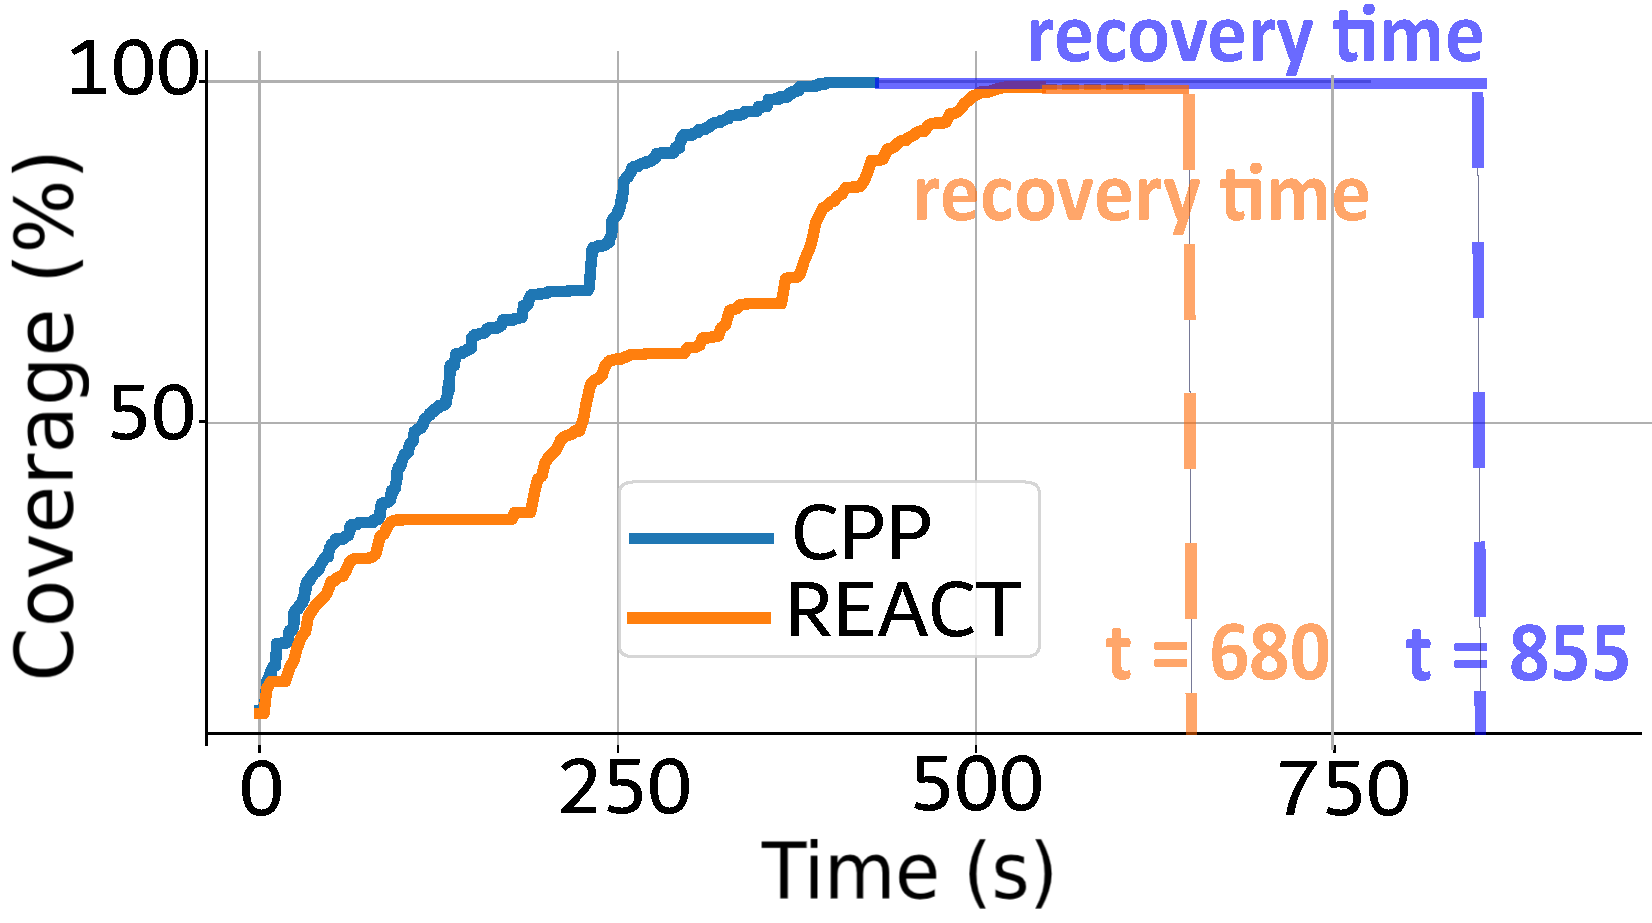
\includegraphics[width=\linewidth]
        {coverage_vs_time_recovery.pdf}
        \caption{Coverage vs. time.}
        \label{fig:coverage_vs_time}
    \end{subfigure}
    \hfill
    \begin{subfigure}[b]{0.48\linewidth}
        \centering
        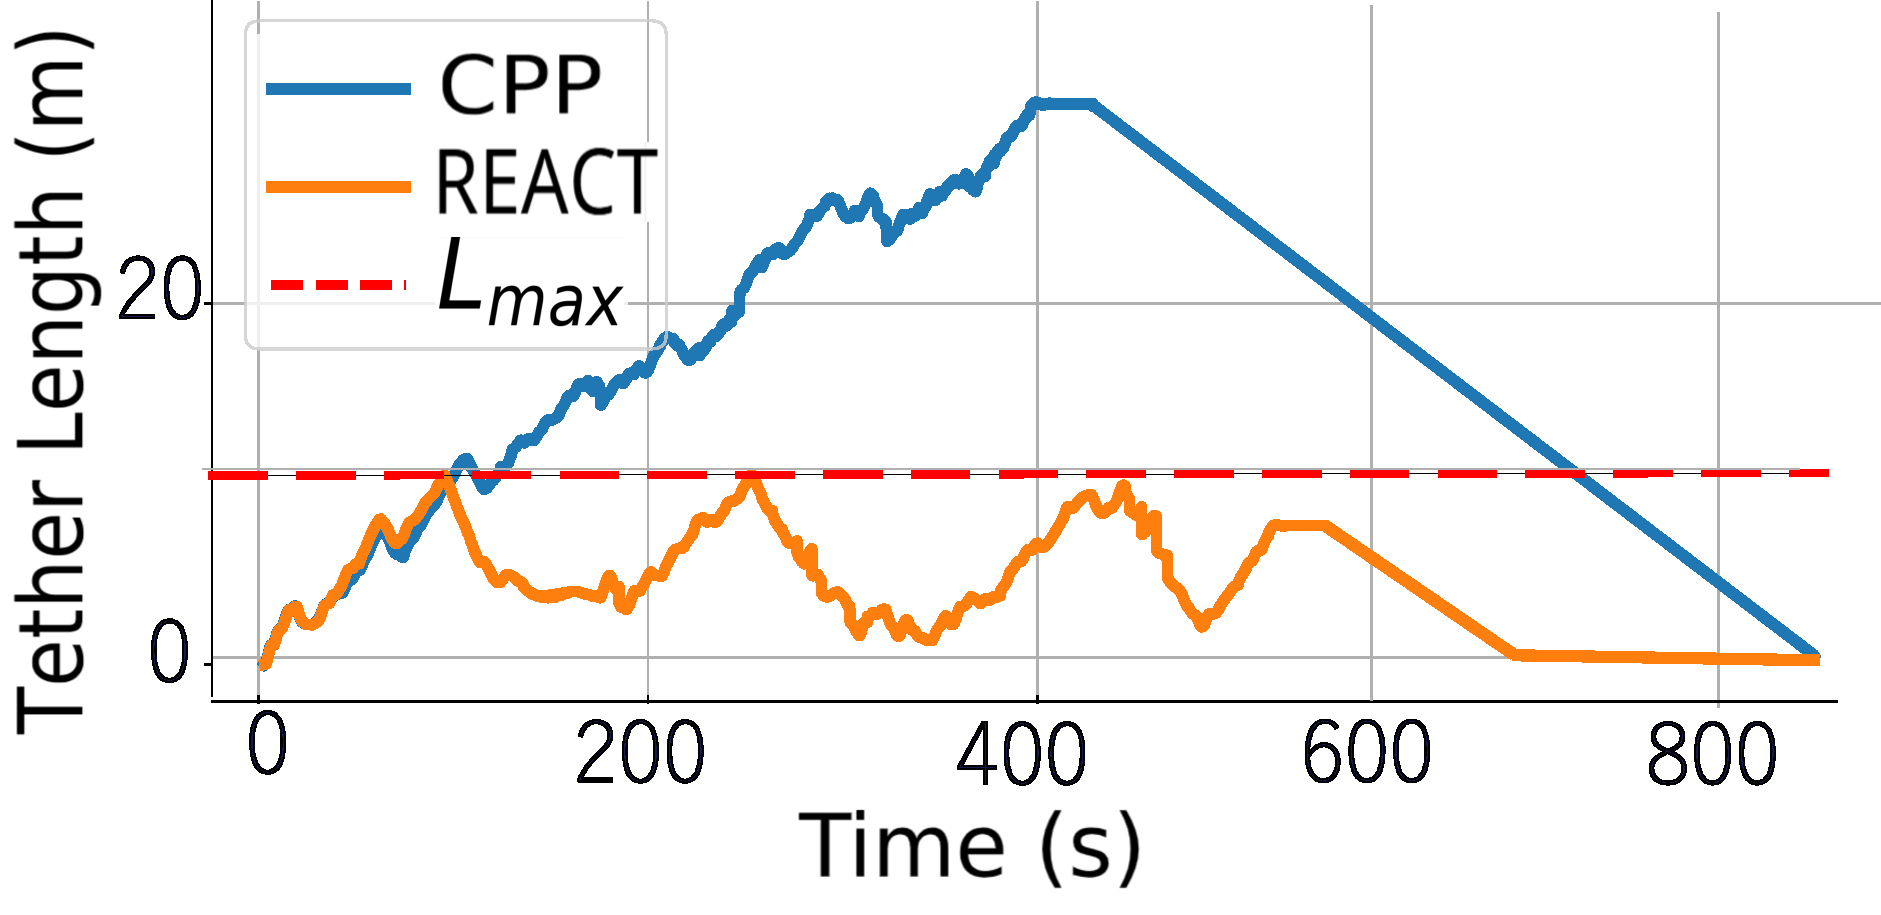
\includegraphics[width=\linewidth]{EA-Planner/figures/tether_length_vs_time_with_recovery.pdf}
        \caption{Tether Length vs. time.}
        \label{fig:tether_vs_time}
    \end{subfigure}
    \caption{Comparison of coverage and tether behavior over time.}
    \label{fig:coverage_tether_sidebyside}
\end{figure}

\begin{figure}[ht]
    \centering
    \begin{subfigure}[b]{0.48\linewidth}
        \centering
        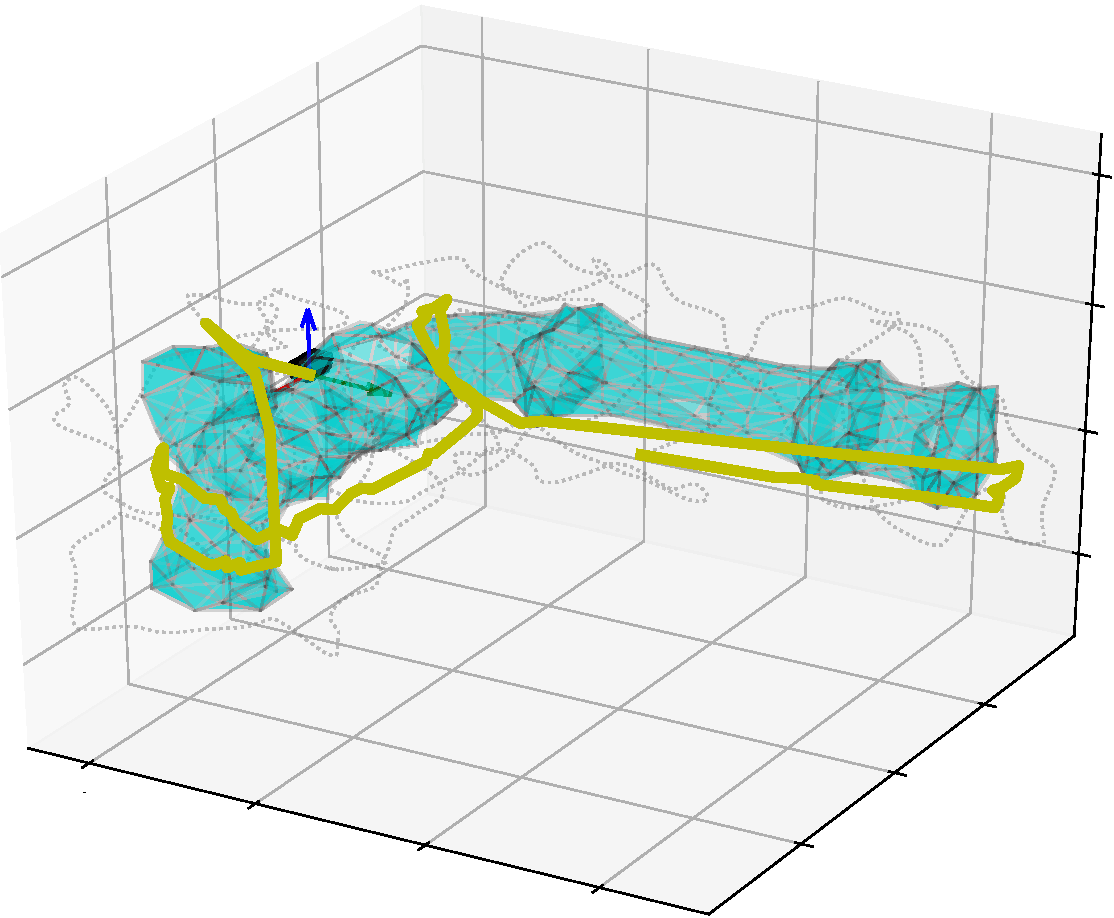
\includegraphics[width=\linewidth]{EA-Planner/figures/fc_planner_final_view.pdf}
        \caption{\ac{CPP} final tether path.}
        \label{fig:3d_cpp}
    \end{subfigure}
    \hfill
    \begin{subfigure}[b]{0.48\linewidth}
        \centering
        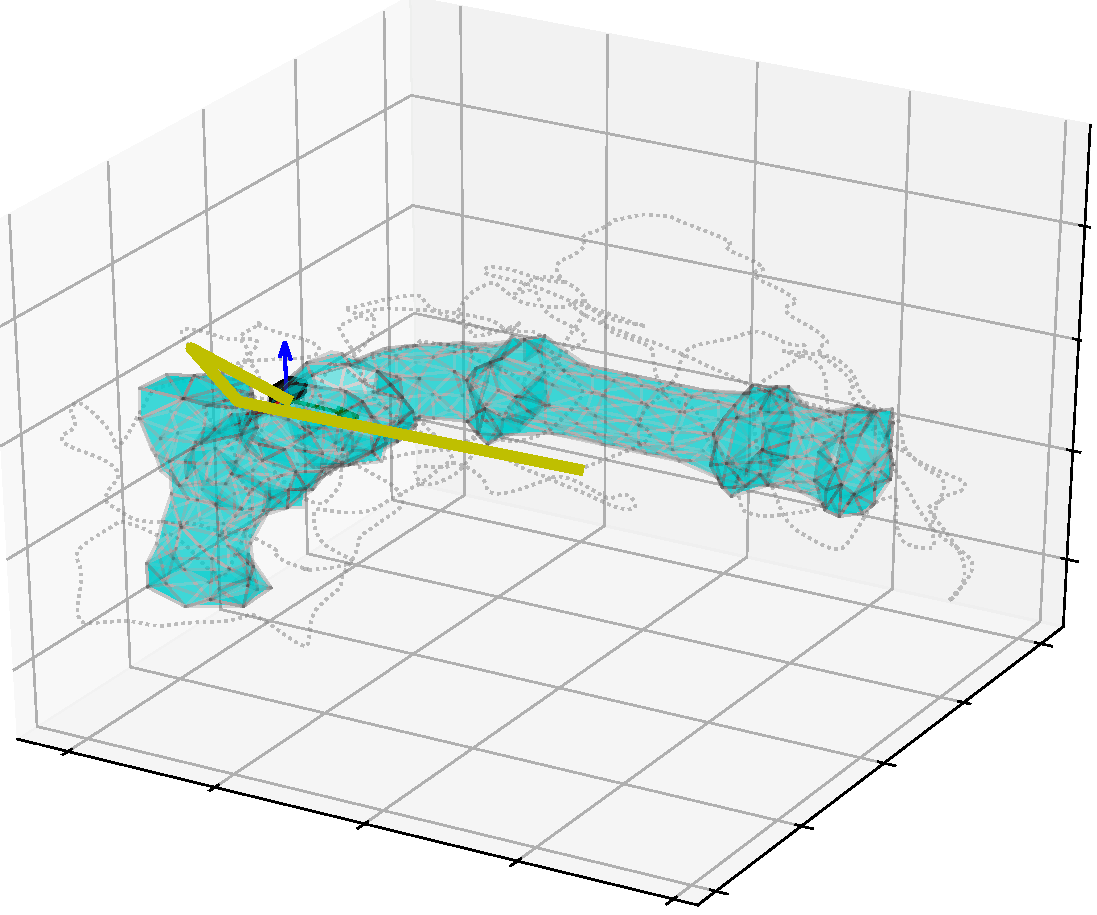
\includegraphics[width=\linewidth]{EA-Planner/figures/react_pipe.pdf}
        \caption{\ac{REACT} final tether path.}
        \label{fig:3d_oea}
    \end{subfigure}
    \caption{3D views of final trajectories. (a) CPP results in entangled tether path. (b) \ac{REACT} yields a non-entangled tether path, reflecting effective entanglement avoidance.}
    \label{fig:3Dplots}
\end{figure}

The performance metrics for both planners are summarized in Table~\ref{tab:performance_metrics} and Table~\ref{tab:tether_metrics}, while Figures~\ref{fig:coverage_tether_sidebyside} and~\ref{fig:3Dplots} visualize the performance of the planners in terms of environmental coverage, tether length behavior, and final trajectory configurations. The evaluation focuses on comparing mission efficiency, constraint compliance, and safety aspects between the entanglement-aware \ac{REACT} method and the conventional \ac{CPP} baseline approach.

The results present two phases: the inspection phase and the recovery phase, where the recovery time represents the estimated duration required to return to the starting position after complete inspection while disentangling the entire tether.

The results highlight distinct trade-offs between the two planning strategies. As shown in Table~\ref{tab:performance_metrics}, the \ac{CPP} method achieves a shorter inspection time (429s vs. 546s) due to its straightforward path execution without rerouting for disentanglement. However, focusing solely on inspection speed overlooks the critical aspect of tether management in constrained environments. The \ac{CPP} exhibits a significantly longer total mission time (855s vs. 680s) because extensive disentanglement is required after inspection completion.

\ac{REACT} demonstrates multiple instances of entanglement detection and resolution, as evidenced by the peaks in the tether length curve in Figure~\ref{fig:tether_vs_time} and the corresponding flat regions in the coverage curve in Figure~\ref{fig:coverage_vs_time}, where the \ac{ROV} inspection progress stops to reroute and find paths without entanglement. This reactive replanning behavior directly results in a longer inspection time, as the system prioritizes tether safety over raw speed.

In particular, the limit on the length of the tether is rarely exceeded by \ac{REACT}, as shown in Table~\ref{tab:tether_metrics} and Fig.~\ref{fig:tether_vs_time}. Conversely, the \ac{CPP} method severely violates this constraint, reaching 31.16m for extended periods (327.37s), risking unrecoverable tether entanglement. The 3D trajectory visualizations in Figure~\ref{fig:3Dplots} further illustrate this difference, showing the entangled tether geometry resulting from \ac{CPP} versus the non-entangled configuration achieved by \ac{REACT}. Therefore, \ac{REACT} demonstrates superior performance for safe tethered \ac{ROV} inspection.
